% Chapter Template

\chapter{Kernel Discriminant Analysis} % Main chapter title
\label{ChapterKernel}

We tackle the dimensionality reduction problem in the context of profiling attacks against implementations protected by masking countermeasure. For such attacks, the attacker might have or not access to the  random values drawn at every execution and used to mask the sensitive variables. If he have such a knowledge, then the dimensionality reduction problem turns to be equivalent to the case of unprotected implementations. Thus ,the classic statistics for the PoIs research (and we will concentrate over the SNR, see Sec.~\ref{sec:extractors}) and the linear dimensionality reduction techniques described in the previous chapter are still applicable and efficient. On the contrary, when such a knowledge is denied, linear techniques are completely inefficient: a non-linear function of the PoIs must considered in order to construct discriminant features from side-channel observations. In this chapter we propose to make use of Kernel Discriminant Analysis (KDA) technique to construct such a non-linear processing. To this aim we revisit the contents and the experimental results of the paper presented at CARDIS 2016 international conference \cite{cagli2016kernel}. After such a publication, the KDA has been compared to other non-linear dimensionality reduction techniques in \cite{manifold}, where manifold learning solutions such as ISOMAP, Locally Linear Embedding (LLE) and Laplacian Eigenmaps (LE) are proposed. Moreover, a use of the KDA in an unsupervised way to perform a higher-order SCA (as a key candidate distinguisher and not as a dimensionality reduction technique) has been proposed at CARDIS 2017 \cite{zhou2017novel}.


%----------------------------------------------------------------------------------------
%	SECTION 1
%----------------------------------------------------------------------------------------

\section{Motivation}
When a masking countermeasure is properly applied, it ensures that every sensitive variable $\sensRandVar$  is randomly split  into multiple shares $M_1,M_2,\dots,M_d$ in such a way that a relation $Z = M_1 \star \dots \star M_d$ holds for a group operation $\star$ (\emph{e.g.} the exclusive or for the Boolean masking). The value $d$ plays the role of a security parameter and the method is usually referred to as $(d-1)$th-order masking (since it involves $d-1$ random values). In many cases, especially for software implementations, the shares are manipulated at different times, and no time sample therefore shows dependency on $\sensRandVar$: in order to recover such  information the attacker is obliged to join information held by each of the $d$ shares, executing a so-called $d$th-order SCA. In the great majority of the published higher-order attacks, the PoI selection during the pre-attack characterization phase is either put aside or made  under the hypothesis that the random shares are known. Actually, the latter knowledge brings the problem back to the unprotected case. 
%, and the methods recalled in previous paragraphs can be directly applied. 
Here we relax this hypothesis and we consider  situations where the values of the random shares are unknown to the adversary. We however assume that the adversary can characterize the leakage before attacking the implementation, by controlling the value of the target variable $\sensRandVar$. These two assumptions put our study in the context of {\em profiling attacks without knowledge of the masks}. \\

\subsection{Getting information from masked implementations}\label{sec:HO}
The SNR estimation defined by \eqref{eq:SNR_formula} is an instrument to measure, point by point, the information held by the first-order moment of the acquisition, \emph{i.e.} the information obtainable observing the variation of the mean of the acquisitions. We refer to such information as a \emph{1st-order information}. In masked implementations, such information is null: in any time sample the mean is independent from $\sensRandVar$ due to the randomization provided by the shares, namely the quantity $\esper[\vaLeakVec\vert \sensRandVar=\sensVar]$, seen as a function of $\sensVar$, is constant, which implies that the SNR is asymptotically  null over the whole trace.\\
 
When a $(d-1)$th-order masking is applied, the information about the shared sensitive target $\sensRandVar$ lies in some $d$th-order statistical moments of the acquisition,\footnote{whence the name {\em $d$th-order attacks}} meaning that for some $d$-tuples of samples $(t_1,\dots ,t_d)$ the quantity $\esper[\vaLeakVec[t_1]\vaLeakVec[t_2]\cdots \vaLeakVec[t_d]\vert \sensRandVar=\sensVar]$ (based on a $d$th-order raw moment) is not constant as a function of $\sensVar$ (equivalently, $ \esper[(\vaLeakVec[t_1]-\esper[\vaLeakVec[t_1]])\cdots (\vaLeakVec[t_d]-\esper[\vaLeakVec[t_d]])\vert \sensRandVar=\sensVar]$ is not constant, using the central moment). We can refer to the information obtainable observing such variation as a {\em $d$th-order information}.
In order to let the SNR reveal it, and consequently let such information be directly exploitable by common attacks, the attacker must pre-process the traces through an extractor $\extract$ that renders the mean of the extracted data dependent on $\sensRandVar$, \emph{i.e.} such that $\esper[\extract(\vaLeakVec)\vert \sensRandVar=\sensVar])$ is not constant as a function of $\sensVar$. In this way, the $d$th-order information is brought back to a $1$st-order one.

\begin{property}[SCA efficiency necessary condition]\label{property:poly}
Let us assume that $\sensRandVar$ is represented by a tuple of shares $M_i$ manipulated at $d$ different times. Denoting $t_1,\dots,t_d$ the time samples\footnote{not necessary distinct} where each share is handled, the output of an effective extractor needs to have at least one coordinate whose polynomial representation over the variables given by the coordinates of $\vaLeakVec$ contains at least one term divisible by the the $d$th-degree monomial $\prod_{i=1,\dots,d}\vaLeakVec[t_i]$ (see \emph{e.g.} \cite{carlet2014achieving} for more information).
\end{property}


\begin{remark}\label{remark:normalized}
The use of central moments has been experimentally shown to reveal more information than the use of the raw ones \cite{chari1999towards,DBLP:journals/tc/ProuffRB09}. Thus we will from now on suppose that the acquisitions have previously been normalized, so that $\esperEst(\vLeakVec_i) = \boldsymbol{0}$ and $\varEst(\vLeakVec_i) = \boldsymbol{1}$. In this way a centred product coincides with a non-centred one. 
\end{remark}

We motivate hereafter through a simplified but didactic  example, the need for a computationally efficient dimensionality reduction technique as preliminary step to perform an higher-order attack.


\subsection{Some strategies to perform higher-order attack}\label{sec:example}
We consider here an SCA targeting an $8$-bit sensitive variable $\sensRandVar$ which has been priorly split into $d$ shares and we assume that a reverse engineering and signal processing have priorly been executed to isolate the manipulation of each share  in a region of $\ell$ time samples. This implies that our SCA  now amounts to extract a $\sensRandVar$-dependent information from leakage measurements whose size has been reduced to $d\times \ell$ time samples. To extract such information three main approaches were proposed in literature until 2016.\\

The first one consists in considering $d$ time samples  at a time, one per region, and in testing if they jointly contain information about $\sensRandVar$ (\emph{e.g.} by estimating the mutual information  \cite{Reparaz2012} or by processing a Correlation Power Attack (CPA) using their centred product \cite{chari1999towards}, etc.). Computationally speaking, this approach requires to evaluate $\ell^d$ $d$-tuples (\emph{e.g.} 6.25 million $d$-tuples for $d=4$ and $\ell=50$), thus its complexity grows exponentially with $d$. \\

The second approach, that avoids the exhaustive enumeration of the $d$-tuples of time samples, consists in estimating the conditional pdf of the whole region: 
to this scope, a Gaussian mixture model is proposed in literature \cite{lemke2007gaussian,Lomne2014} and the parameters of such a Gaussian mixture can be estimated through the expectation-maximization (EM) procedure. In \cite{lemke2007gaussian} 4 variants of the procedure are proposed according to a trade-off between the efficiency and the accuracy of the estimations;  the most rough leads to the estimation of  $256^{(d-1)}(\ell d)$  parameters (\emph{e.g.} $\approx 3.4 $ billion parameters for $d=4$ and $\ell=50$), while the finest one requires the estimation of $256^{(d-1)}(1 + \frac{3\cdot \ell d}{2} + \frac{(\ell d)^2}{2}-1)$ parameters (\emph{e.g.} $\approx 87$ trillion parameters). Once again, the complexity of the approach grows exponentially with the order $d$.\\

The third approach, whose complexity does not increase exponentially with $d$, is the application of the higher-order version of the PP tool for the PoI selection, for which we give an outline hereafter. As will be discussed in Sec.~\ref{sec:comparisonPP}, its heuristic nature is the counterpart of the relatively restrained complexity of this tool. \\

%

\subsubsection{Higher-Order Version of Projection Pursuits}\label{sec:PP_description}
The $d$th-order version of PP makes use of the so-called \emph{Moment against Moment Profiled Correlation} (MMPC) as objective function. The extractor $\extract^{PP}$ has the following form:
\begin{equation} 
\extract^{PP}(\vLeakVec) = (\AAlpha\cdot\vLeakVec)^d \mbox{ ,}
\end{equation}
where $\AAlpha$ is a sparse projecting vector with $d$ non-overlapping windows of coordinates set to 1, in correspondence with the identified points of interest. Actually, as will be discussed in Sec.~\ref{sec:comparisonPP}, authors of \cite{PP} propose to exploit $\AAlpha$ as a pointer of PoIs, but do not encourage the use of $\extract^{PP}$ as an attack preprocessing. The procedure is divided into two parts: a global research called {\em Find Solution} and a local optimization called {\em Improve Solution}. At each step of {\em Find Solution}, $d$ windows are randomly selected to form a primordial $\AAlpha$, thus a primordial $\extract^{PP}$. A part of the training traces are then processed via $\extract^{PP}$ and used to estimate the $d$th-order statistical moments $\mmm^d_\sensVar = \esperEst_i[(\extract^{PP}(\vLeakVec_i))_{i:\sensVar_i=\sensVar}])$,  for each value of $\sensVar$. Then the Pearson correlation coefficient $\hat{\rho}$ between such estimates and the same estimates issued from a second part of the training set is computed. If $\hat{\rho}$ is higher than some threshold $T_{det}$, the windows forming $\AAlpha$ are considered interesting\footnote{A further validation is performed over such windows, using other two training sets to estimate $\hat{\rho}$, in order to reduce the risk of false positives.}\label{fn:4trainingSets} and \emph{Improve Solution} optimises their positions and lengths, via small local movements. Otherwise, the $\AAlpha$ is discarded and another $d$-tuple of random windows is selected.\\

The threshold $T_{det}$ plays a fundamental role in this crucial part of the algorithm: it has to be small enough to promote interesting windows (avoiding false negatives) and high enough to reject uninteresting ones (avoiding false positives). A hypothesis test is used to choose a value for $T_{det}$ in such a way that the probability of $\hat{\rho}$ being higher than $T_{det}$ given that no interesting windows are selected is lower than a chosen significance level $\beta$.\footnote{Interestingly, the threshold $T_{det}$ depends on size of $\sensVarSet$ and not on the size of the training sets of traces. This fact disables the classic strategy that consists in enlarging the sample, making $T_{det}$ lower, in order to raise the statistical power of the test (\emph{i.e.} $\mathrm{Prob}[\hat{\rho}>T_{det}\vert \rho=1]$). Some developments of this algorithm have been proposed \cite{durvauximproved}, also including the substitution of the MMPC objective function with a \emph{Moments against Samples} one, that would let $T_{det}$ decrease when increasing the size of the training set.} \\

\subsection{Foreword of this study}

The exploitation of KDA technique in the way we propose in this chapter aims to exploit interesting $d$-tuples of time samples as the first strategy described in Sec.~\ref{sec:example}. It however improves it in several aspects. In particular, its complexity does not increase exponentially with $d$. Moreover, it may be remarked that such a first approach allows the attacker to extract interesting $d$-tuples of points, but does not provide any hint to conveniently combine them. This is an important limitation since  finding a convenient way to combine time samples would raise the SCA efficiency, as already experimentally shown in \cite{boosting}, for $d = 1,2$. Nevertheless in the SCA literature no specific method has been proposed for the general case $d>2$.  This study aims to propose a new answer to this question, while showing that it compares favourably to the PP approach.

%\subsection{Our Contribution}
%The ideas developed in the paper are based on the so-called Kernel Discriminant Analysis (KDA) \cite{hofmann2008kernel,scholkopf1999fisher}, which essentially consists in applying a so-called \emph{kernel trick} to the LDA. The trick is a stratagem that allows performing the LDA over a higher-dimensional \emph{feature space} (whose dimension can even raise exponentially with $d$) in which information about $Z$ lies in single dimensions and can be enhanced through linear combinations, keeping the computational cost independent from the dimension of the feature space (thus independent from $d$).\footnote{Even if the complexity is independent of $d$, the amount of information extracted is still decreasing exponentially with $d$, as expected when $(d-1)$-th order masking is applied \cite{chari1999towards}.} This study is in line with other recent works aiming to apply machine learning techniques to the side-channel context, such as \cite{machineLearningSCA,lerman2015template} which also exploit kernel functions to deal with non-linearly separable data.\\

%We show that the application of the KDA comes with several issues that we identify and analyse.
%We afterwards apply it to attack  masked operations implemented over an 8-bit AVR microprocessor Atmega328P. The experiments performed in $2$nd-order, $3$rd-order and $4$th-order contexts confirm the effectiveness of the KDA: in all cases the dimensionality reductions provided by the KDA lead to efficient and successful key recovery template attacks.\\



%The paper is organised as follows: in Sec.~\ref{sec:general} the notations are established, together with the formalization of the treated problem.  Moreover, some State-of-the-Art methods, efficient for the $1$st-order context, are recalled. In Sec.~\ref{sec:KDA}, the KDA method is described. A discussion about issues related to the application of the KDA to the SCA is conducted in Sec.~\ref{sec:practice} on the basis of experimental results. Finally, a comparison with the PP approach is proposed in Sec.~\ref{sec:PP}.

%----------------------------------------------------------------------------------------
%	SECTION 2
%----------------------------------------------------------------------------------------

\section{Feature Space, Kernel Function and Kernel Trick}\label{sec:kernel_trick}


As described in Sec.~\ref{sec:HO}, the hard part of the construction of an effective extractor  is the detection of $d$ time samples $t_1,\dots,t_d$ where the shares leak. A naive solution, depicted in Fig.~\ref{fig:scheme1}, consists in applying to the traces the centred product preprocessing for each $d$-tuple of time samples. Formally it means immerse the observed data in a higher-dimensional space, via a non-linear function
\begin{equation}\label{eq:featureSpace}
\Phi \colon \mathbb{R}^\traceLength \rightarrow \featureSpace = \mathbb{R}^{{D+d-1}\choose{d}} \mbox{ .}
\end{equation}
 Using the Machine Learning language the higher-dimensional space $\featureSpace$ will be called \emph{feature space}, because in such a space the attacker finds the features that discriminate different classes. Procedures involving a feature space defined as in \eqref{eq:featureSpace} imply the construction, the storage and the management of ${D+d-1}\choose{d}$-sized traces; such a combinatorially explosion of the size of $\featureSpace$ is undoubtedly an obstacle from a computational standpoint.
 
\begin{figure}
\centering
{
\begin{tikzpicture}
\matrix (m) [matrix of math nodes, row sep=3em,
column sep=3em, text height=1.5ex, text depth=0.25ex]
{ \mathbb{R}^\traceLength & \featureSpace & \mathbb{R}^\newTraceLength \\};
\path[->]
(m-1-1) edge node[above] {$\Phi$} (m-1-2);
         %edge [bend left=30] (m-2-2)
         %edge [bend right=15] (m-2-2);
\path[->]
($(m-1-2.north east)-(0,0.1)$) edge node[above] {$\extract^{\mathrm{PCA}}$} ($(m-1-3.north west)-(0,0.1)$);
\path[->]
($(m-1-2.south east)+(0,0.15)$) edge node[below] {$\extract^{\mathrm{LDA}}$} ($(m-1-3.south west)+(0,0.15)$);

\end{tikzpicture} 
}
\caption{Performing LDA and PCA over a high-dimensional feature space.}\label{fig:scheme1}
\end{figure} 
 
 In Machine Learning a stratagem known as \emph{kernel trick} is available for some linear classifiers, such as Support Vector Machine (SVM), PCA and LDA, to turn them into non-linear classifiers, providing an efficient way to implicitly compute them into a high-dimensional feature space. This section gives an intuition about how the kernel trick acts. It explains how it can be combined with the LDA, leading to the so-called KDA algorithm, that enables an attacker to construct some non-linear extractors that concentrate in few points the $d$-th order information held by the side-channel traces, without requiring computations into a high-dimensional feature space, see Fig.~\ref{fig:scheme2}. 

\begin{figure}
\centering
{
\begin{tikzpicture}
\matrix (m) [matrix of math nodes, row sep=3em,
column sep=3em, text height=1.5ex, text depth=0.25ex]
{ \mathbb{R}^\traceLength & \featureSpace & \mathbb{R}^\newTraceLength \\};
\path[->]
(m-1-1) edge node[above] {$\Phi$} (m-1-2);
         %edge [bend left=30] (m-2-2)
         %edge [bend right=15] (m-2-2);
\path[->]
($(m-1-2.north east)-(0,0.1)$) edge node[above] {$\extract^{\mathrm{PCA}}$} ($(m-1-3.north west)-(0,0.1)$);
\path[->]
($(m-1-2.south east)+(0,0.15)$) edge node[below] {$\extract^{\mathrm{LDA}}$} ($(m-1-3.south west)+(0,0.15)$);

\path[->]
(m-1-1) edge [bend left=50] node[above] {$\extract^{\mathrm{KPCA}}$} (m-1-3)
(m-1-1) edge [bend right=50] node[below] {$\extract^{\mathrm{KDA}}$} (m-1-3);

\end{tikzpicture} 
}
\caption{Applying KDA and KPCA permits to by-pass computations in $\featureSpace$.}\label{fig:scheme2}
\end{figure}

The central tool of a kernel trick is the \emph{kernel function} $K \colon \mathbb{R}^\traceLength \times \mathbb{R}^\traceLength \rightarrow \mathbb{R}$, that has to satisfy the following property, in relation with the function $\Phi$:

\begin{equation}\label{eq:kernelProperty}
K(\vLeakVec_i,\vLeakVec_j) = \Phi(\vLeakVec_i)\cdot \Phi(\vLeakVec_j) \mbox{ ,}
\end{equation}
for each $i,j= 1,\dots, \nbTraces$, where $\cdot$ denote the dot product.


Every map $\Phi$ has an associated kernel function given by \eqref{eq:kernelProperty}, for a given set of data. The converse is not true: all and only the functions $K\colon\mathbb{R}^D\times \mathbb{R}^D \rightarrow \mathbb{R}$ that satisfy a convergence condition known as {\em Mercer's condition} are associated to some map $\Phi:\mathbb{R}^D	\rightarrow \mathbb{R}^\featureSpaceSize$, for some $\featureSpaceSize$. Importantly, a kernel function is interesting only if it is computable directly from the rough data $\vLeakVec$, without evaluating the function $\Phi$. \\

The notion of kernel function is illustrated in the following example.

\begin{example}\label{ex:polyKernel}
Let $D=2$. Consider the function
\begin{align}
&K\colon\mathbb{R}^2\times \mathbb{R}^2 \rightarrow \mathbb{R} \nonumber \\ 
&K\colon(\vLeakVec_i,\vLeakVec_j) \mapsto ( \vLeakVec_i\cdot \vLeakVec_j)^2 \mbox{ ,} \label{eq:example1}
\end{align}

After defining $\vLeakVec_i = [a,b]$ and $\vLeakVec_j = [c,d]$, we get the following development of K:
\begin{equation}
K(\vLeakVec_i,\vLeakVec_j) = (ac + bd)^2 = a^2c^2 + 2abcd + b^2d^2 \mbox{ ,}
\end{equation}

which is associated to the following map from $\mathbb{R}^2$ to $\featureSpace \subset\mathbb{R}^3$:
\begin{equation}
\Phi(u,v) =  [u^2, \sqrt{2}uv, v^2]
\end{equation}

Indeed $\Phi(\vLeakVec_i)\cdot \Phi(\vLeakVec_j) = a^2c^2 + 2abcd + b^2d^2 = K(\vLeakVec_i,\vLeakVec_j)$\enspace. This means that to compute the dot product between some data mapped into the $3$-dimensional space $\featureSpace$ there is no need to apply $\Phi$: applying $K$ over the $2$-dimensional space is equivalent. This trick allows the short-cut depicted in Fig.~\ref{fig:scheme2}.

\end{example}



In view of the necessary condition exhibited by Property~\ref{property:poly},  the function $K(\vLeakVec_i,\vLeakVec_j) = (\vLeakVec_i \cdot \vLeakVec_j)^d$, hereafter named \emph{$d$th-degree polynomial kernel function}, is the convenient choice for an attack against implementations protected with $(d-1)$th-order masking. It corresponds to a function $\Phi$ that brings the input coordinates into a feature space $\featureSpace$ containing all possible $d$-degree monomials in the coordinates of $\vLeakVec$, up to constants. This is, up to constants, exactly the $\Phi$ function of \eqref{eq:featureSpace}.\footnote{Other polynomial kernel functions may be more adapted if the acquisitions are not free from $d^\prime$th-order leakages, with $d^\prime<d$. Among non-polynomial kernel functions, we effectuated some experimental trials with the most common Radial Basis Function (RBF), obtaining no interesting results. This might be caused by the infinite-dimensional size of the underlying feature space, that makes the discriminant components estimation less efficient.}\\ 

%----------------------------------------------------------------------------------------
%	SECTION 3
%----------------------------------------------------------------------------------------

\section{Kernel Discriminant Analysis}
The equation \eqref{eq:kernelProperty} shows that a kernel function $K$ allows to compute the dot product between elements mapped into the feature space $\featureSpace$ \eqref{eq:kernelProperty}. By extension, any procedure that only implies the computation of dot products between elements of $\featureSpace$, can be executed exploiting a kernel function. Starting from this remark, the authors of  \cite{scholkopf1998nonlinear,scholkopf1999fisher} have shown that the PCA and LDA procedures can be adapted to satisfy the latter condition, which led them to define the KPCA and KDA algorithms. The latter one is described in Sec.~\ref{sec:KDA}. The interested reader will find the formal derivation of KPCA in Appendix~\ref{app:KPCA}, reported as a way of example of how one can translate the classical PCA algorithm (and the class-oriented version) in such a way to never access data, but only dot product between data. The way to derive the KDA procedure reported below is analogous; the interested reader might refer to \cite{scholkopf1999fisher}, or to \cite{baudat2000generalized} for the multi-class version.

\subsection{KDA for $d$th-order masked side-channel traces}\label{sec:KDA}
Given a set of labelled training side-channel traces $(\vLeakVec_i, \sensVar_i)_{i=1, \dots , \nbTraces}$ and the kernel function $K(\vLeakVec,\yyy)= (\vLeakVec \cdot \yyy)^d$:
\begin{itemize}

\item[1)] Construct a matrix $\MMM$ (acting as \emph{between-class scatter matrix}):

\begin{equation}
\MMM = \sum_{\sensVar\in\sensVarSet}\nbTracesPerClass(\MMMclass - \MMMT)(\MMMclass-\MMMT)^\intercal\mbox{ ,}
\end{equation}

where $\MMMclass$ and $\MMMT$ are two $N$-sized column vectors whose entries are given by:
\begin{align}
\MMMclass[\sensVar][j] = \frac{1}{\nbTracesPerClass}\sum_{i:\sensVar_i=\sensVar}^{\nbTracesPerClass}K(\vLeakVec_j,\vLeakVec_i)\\
\MMMT[j] = \frac{1}{\nbTraces}\sum_{i=1}^{\nbTraces}K(\vLeakVec_{j},\vLeakVec_{i}) \mbox{ .}
\end{align}


\item[2)] Construct a matrix $\NNN$ (acting as \emph{within-class scatter matrix}):

\begin{equation}\label{eq:N}
\NNN = \sum_{\sensVar\in\sensVarSet}\kernelMatrix_\sensVar(\III - \III_{\nbTracesPerClass})\kernelMatrix_\sensVar^\intercal\mbox{ ,}
\end{equation}
where $\III$ is a $\nbTracesPerClass \times \nbTracesPerClass$ identity matrix, $\III_{\nbTracesPerClass}$ is a $\nbTracesPerClass \times \nbTracesPerClass$ matrix with all entries equal to $\frac{1}{\nbTracesPerClass}$ and $\kernelMatrix_{\sensVar}$ is the $\nbTraces \times \nbTracesPerClass$ sub-matrix of $\kernelMatrix = (K(\vLeakVec_i,\vLeakVec_j))_{\substack{i=1,\dots,\nbTraces \\ j=1,\dots,\nbTraces}}$ storing only columns indexed by the indices $i$ such that $\sensVar_i=\sensVar$. 

\item[3)] Regularize the  matrix $\NNN$ for computational stability:
\begin{equation}\label{eq:mu}
\NNN = \NNN + \mu  \III \quad \mbox{ see \ref{sec:mu};}
\end{equation}

\item[4)]\label{point:eigs} Find the non-zero eigenvalues $\lambda_1, \dots, \lambda_\numEigenvectors$ and the corresponding eigenvectors $\nununu_1, \dots, \nununu_\numEigenvectors$ of $\NNN^{-1}\MMM$; 


\item[5)] Finally, the projection of a new trace $\vLeakVec$ over the $\ell$-th non-linear $d$th-order discriminant component can be computed as:
\begin{equation}\label{eq:projectionKDA}
\extract^{\mathrm{KDA}}_{\ell}(\vLeakVec) = \sum_{i=1}^{\nbTraces}\boldsymbol{\nu}_\ell[i]K(\vLeakVec{i}, \vLeakVec) \mbox{ .}
\end{equation} 

\end{itemize}
For the reasons discussed in Sec.~\ref{sec:kernel_trick}, the right-hand side of \eqref{eq:projectionKDA} may be viewed as an efficient way to process the $\ell$th coordinate of the vector $\extract^{LDA}(\Phi(\vLeakVec))[\ell] = \www_{\ell} \cdot \Phi(\vLeakVec)$,
without evaluating $\Phi(\vLeakVec)$. The entries of $\www_{\ell}$ are never computed, and will thus be referred to as \emph{implicit coefficients} (see Sec.~\ref{sec:implicit} below). It may be observed that each discriminant component $\extract^{\mathrm{KDA}}_{\ell}(\cdot)$ depends on the training set $(\vLeakVec_i, \sensVar_i)_{i=1, \dots , \nbTraces}$, on the kernel function $K$ and on the regularization parameters $\mu$.

\subsection{The implicit coefficients}\label{sec:implicit}
As already said, when the $d$th-degree  polynomial kernel function is chosen as kernel function, the KDA operates implicitly in the feature space of all products of $d$-tuples of time samples. In order to investigate the effect of projecting a new trace $\vLeakVec$ over a component $\extract^{\mathrm{KDA}}_{\ell}(\vLeakVec)$, we can compute for a small $d$ the implicit coefficients that are assigned to the $d$-tuples of time samples through \eqref{eq:projectionKDA}. For $d=2$ we obtain that in such a feature space the projection is given by the linear combination computed via the coefficients shown below: 
\begin{equation}\label{eq:implicit}
\extract^{\mathrm{KDA}}_{\ell}(\vLeakVec) = \sum_{j=1}^\traceLength \sum_{k=1}^\traceLength[ (\vLeakVec[j]\vLeakVec[k])\underbrace{(\sum_{i=1}^{\nbTraces}\boldsymbol{\nu}_{\ell}[i] \vLeakVec_i[j]\vLeakVec_{i}[k])}_{\mbox{implicit \ coefficients}}]
\end{equation}




\subsection{Computational complexity analysis}
The order $d$ of the attack does not significantly influence the complexity of the KDA algorithm. Let $\nbTraces$ be the size of the training trace set and let $D$ be the trace length, then the KDA requires:
\begin{itemize}
\item $\frac{\nbTraces^2}{2}D$ multiplications, $\frac{\nbTraces^2}{2}(D-1)$ additions and $\frac{\nbTraces^2}{2}D$ raising to the $d$-th power, to process the kernel function over all pairs of training traces
\item $(D+C)$ multiplications, $(D+C-2)$ additions and 1 raising to the $d$-th power for the projection of each new trace over $C$ KDA components,
\item the cost of the eigenvalue problem, that is $O(\nbTraces^3)$.
\end{itemize} 

In next sections we discuss the practical problems an attacker has to deal with when applying the KDA. The argumentation is conducted on the basis of experimental results whose setup is described hereafter.

%----------------------------------------------------------------------------------------
%	SECTION 4
%----------------------------------------------------------------------------------------
\section{Experiments over Atmega328P}\label{sec:practice}
\subsection{Experimental Setup}\label{sec:experimental_setup}
The target device is an 8-bit AVR microprocessor Atmega328P and we acquired power-consumption traces thanks to the ChipWhisperer platform \cite{o2014chipwhisperer}.\footnote{This choice has been done to allow for reproducibility of the experiments.} From the acquisitions we extracted some traces composed of 200 time samples, corresponding to 4 clock cycles (see Fig.\ref{fig:PP2} or \ref{fig:PP3} upper parts). Depending on the attack implementation, we ensure that the acquisitions contain either 2,3 or 4 shares respectively for $d=2,3$ or $4$. The shares satisfy $M_1 \oplus \dots \oplus M_d = \sensRandVar$,
where $\sensRandVar$ takes values in $\sensVarSet = \mathbb{F}_2^8$ and represents one byte of the output of the first rount SubByte operation in AES: $\sensRandVar = \Sbox(P\oplus \keyRandVar^\star)$. The goal of the attack is to recover the subkey $K^\star$. The plaintext $P$ is assumed to be known and the $M_i$ are assumed to be unknown random uniform values. The profiling phase is divided in two sub-phases that exploit two distinct datasets. The first sub-phase, that we will refer to as KDA training phase, aims at constructing the dimensionality reduction function by means of KDA algorithm. It exploits a KDA dataset $\setDataTrain = (\setLeakTrain,\setTargetTrain)$ of size $\nbTraces=8960$.  A known fixed subkey is used to acquire such a dataset, the plaintexts have been chosen to balance the number of classes ($\nbTracesPerClass=\frac{8960}{256}=35$  for each $\sensVar\in \sensVarSet$).  We fixed the dimension $\newTraceLength$  at the value $2$ (except for the 2-class KDA for which we chose $C=1$, see Remark~\ref{rem:numComp}): we therefore tried to build extractors $\extract^{\mathrm{KDA}}(\cdot) = (\extract^{\mathrm{KDA}}_1(\cdot), \extract^{\mathrm{KDA}}_2(\cdot))$ mapping traces of size 200 samples into new traces composed of 2 coordinates.\footnote{As we have seen in Chapter~\ref{ChapterLinear}, for PCA and LDA methods a good component selection is fundamental to obtain an efficient subspace, and that the first components not always represent the best choice. This is likely to be the case for the KDA as well, but in our experiments the choice of the two first components $\extract^{\mathrm{KDA}}_1, \extract^{\mathrm{KDA}}_2$ turns out to be satisfying, and therefore to simplify our study we preferred to not investigate other choices.} Afterwards, a bivariate Gaussian TA (see Sec.~\ref{sec:TA}) is run. Such an attack demands for a proper profiling phase, consisting in the estimation of the  class-conditional probabilities. It justifies the second profiling sub-phase anticipated above. It will be referred to as profiling phase and will be performed exploiting a distinct profiling dataset  $\setDataProfiling = (\setLeakProfiling,\setTargetProfiling)$, collecting 1000 traces per class, under a fixed known key. The choice of not reusing $\setDataTrain$ as profiling dataset for the Gaussian TA has been done in order to reduce the overfitting risk, discussed in general in Sec.~\ref{sec:overfitting} and that will be discussed in the particular case of KDA in Sec.~\ref{sec:mu}. The extractor $\extract^{\mathrm{KDA}}$, has a different behaviour when applied to the traces used to train it and to some new traces: this is inevitable since $\extract^{\mathrm{KDA}}$ uses all training traces has its proper parameters \eqref{eq:projectionKDA}. Thus, a new unobserved profiling set is mandatory in order to obtain an uncorrupted profiling.
\\

As discussed in Remark~\ref{remark:normalized}, the KDA training traces are normalized. The average trace and the standard deviation trace used to perform the normalization are stored and reused to center the profiling and attack traces before projecting them onto the KDA components. In this way the profiling and attack traces present a form as similar as possible to the training ones.

\subsection{The Regularization Problem}\label{sec:mu}


\begin{figure}
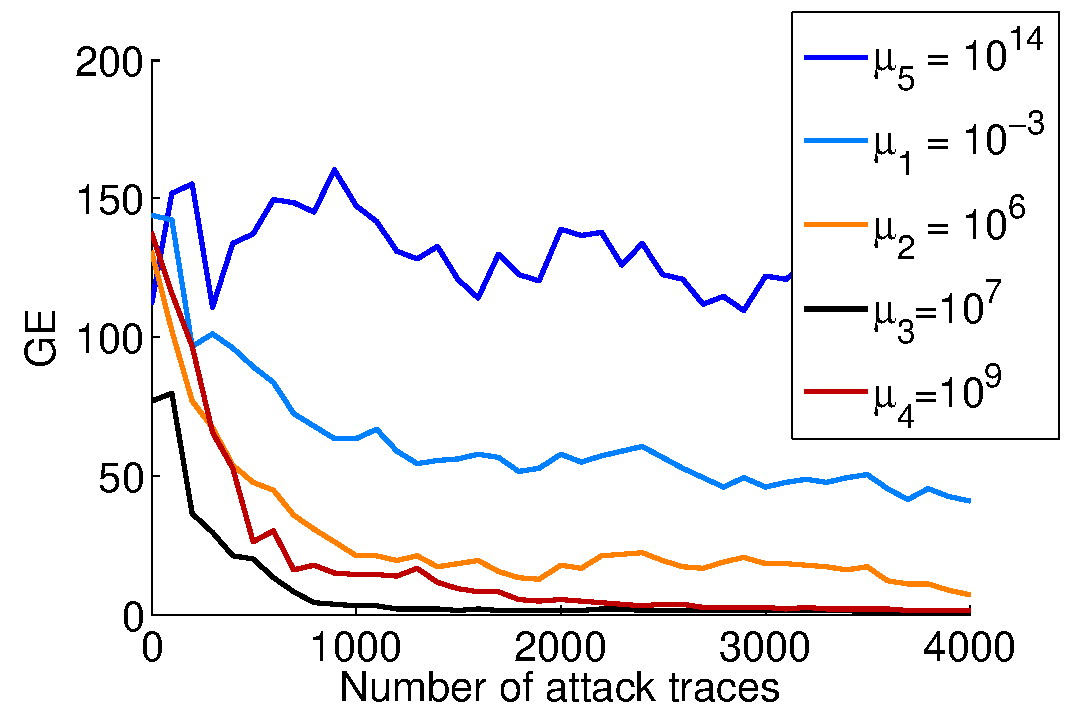
\includegraphics[width=.5\textwidth]{../Figures/CARDIS2016/mu_comparison_new.pdf} 
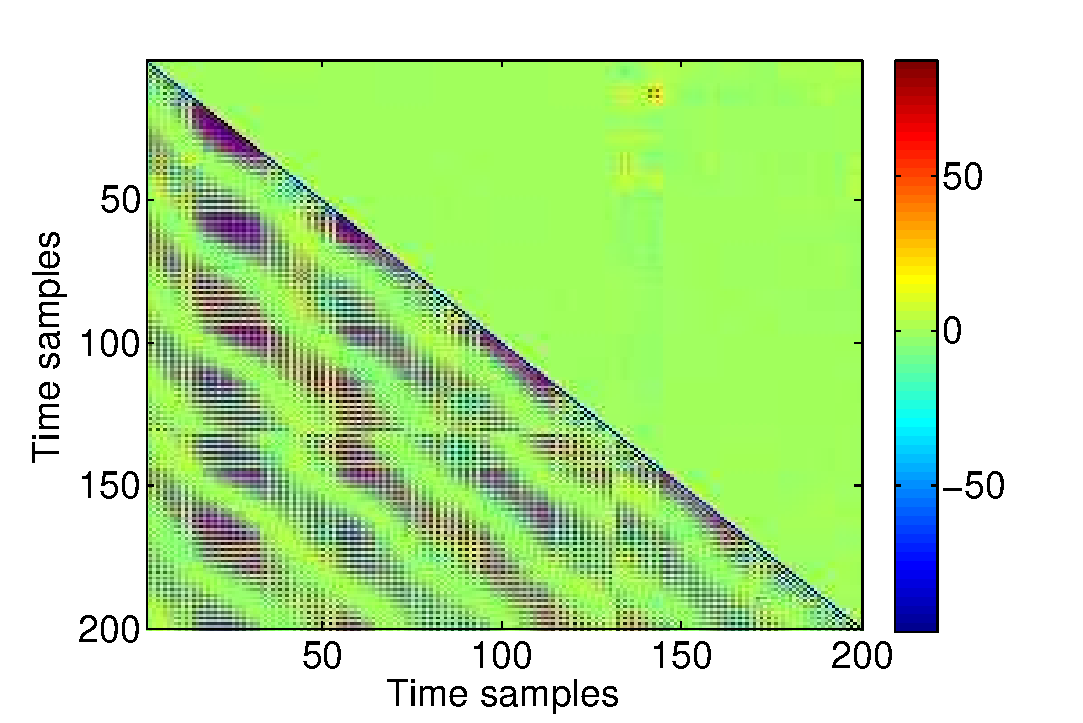
\includegraphics[width=.5\textwidth]{../Figures/CARDIS2016/good_bad_coeffs.pdf} 
\caption[Dependence of KDA performances on the regularization parameter $\mu$. Implicit coefficients.]{On the left: template attack guessing entropy vs the number of traces for the attack phase, varying for choices of the constant $\mu$  \eqref{eq:mu}. On the right: the implicit coefficients assigned to pairs of time samples for $\mu_3$ (upper triangular part) and $\mu_5$ (lower triangular part). }\label{fig:mu}
\end{figure}


By construction the matrix $\NNN$ in \eqref{eq:N} is not positive-definite, which is one of the reasons why in \cite{scholkopf1999fisher}, where the application of a kernel trick to LDA is proposed for the first time, the authors propose the regularization \eqref{eq:mu} recalled hereafter:
\begin{equation}
\NNN = \NNN + \mu\III \mbox{ .}
\end{equation}

When applying such a regularization, the choice of the constant $\mu$ is crucial. Beyond the form of the kernel function, $\mu$ is the unique hyper-parameter of the model constructed by the KDA algorithm, in the sense explained in Sec.~\ref{sec:validation}. Its value cannot be learned from data and has to be priorly fixed somehow. For sure it has to be large enough to ensure that $\NNN$ turns to a positive-definite matrix, but we experimentally observed  that the minimal $\mu$ for which the positive-definitiveness of $\NNN$ is attained is often far from  being the one that provides a good extractor. In Fig.~\ref{fig:mu} (left) we observe the efficiency of a template attack run in combination with a KDA extractor. The matrix $\NNN$ is positive-definite for $\mu_1 = 10^{-3}$ but the value that provides the best extractor is much higher (namely $\mu_3 = 10^{7}$). Still raising the value of $\mu$ degrades the quality of the extractor. The right part of Fig.~\ref{fig:mu} shows the implicit coefficients of the extractor (see \eqref{eq:implicit}) obtained under $\mu_3$ (upper triangular part) and under $\mu_5$ (lower triangular part). The extractor corresponding to the former one leads to a successful attack and has high values concentrated over the interesting windows; the extractor corresponding to the latter one leads to an unsuccessful attack and shows lack of localization around interesting parts of the trace, highlighting the fact that the KDA tool failed in detecting generalisable class-distinguishing features in this case.\\

The regularization \eqref{eq:mu} is a proper regularization in the sense discussed in Sec.~\ref{sec:overfitting}: it is not only a way to make the problem computationally stable (which explains why the minimal $\mu$ making $\NNN$ positive-definite may not be a good choice), but also a answer to the overfitting phenomenon. In the case of the KDA the overfitting is observable when $\extract^{\mathrm{KDA}}$ almost perfectly separates the training traces in their classes, while failing in separating the profiling and the attack ones. In \cite{scholkopf1999fisher} it is shown that the regularization \eqref{eq:mu} corresponds to the additional requirement for $\nununu$ to have a small norm $\lVert\nununu\rVert^2$. As every regularization technique, it makes the method less accurate in the learning phase, but in some cases more likely to correctly operate on new examples.

\begin{remark}
Another regularization strategy may be to search for sparse vectors of implicit coefficients (see \eqref{eq:implicit}). This alternative might be more suitable for the side-channel context, since it would promote localized solutions, \emph{i.e.} projections for which only a few $d$-tuples of time samples contribute to the construction of the extractor (see Assumption \ref{assum:local} in Chapter~\ref{ChapterLinear} for an analogy in $1st$-order context). This approach is left for future developments.
\end{remark} 


Some heuristics exist to choose the constant $\mu$, \eg the average of the diagonal entries \cite{multiclassLDA} or the minimal constant that let $\NNN$ be diagonally dominant (implying positive-definite). In \cite{centeno2006optimising} Centeno \emph{et al.} propose a maximization strategy to find the optimal regularization parameter, based on a probabilistic approach. We did not apply such heuristics for our study, but we consider them in order to fix a grid of values for $\mu$ to be tested. Then, as explained in Sec.~\ref{sec:validation} we chose an approach based over a validation, in order to fix the final value of $\mu$ before performing the attack phase. To perform such validation we chose the SNR as performance measure for the extractor provided by the KDA and $\setDataProfiling$ as validation dataset.


\subsection{The Multi-Class Trade-Off}\label{sec:multiclass}

\begin{figure}[t]
\subfigure[]{\label{fig:numClasses-2order}
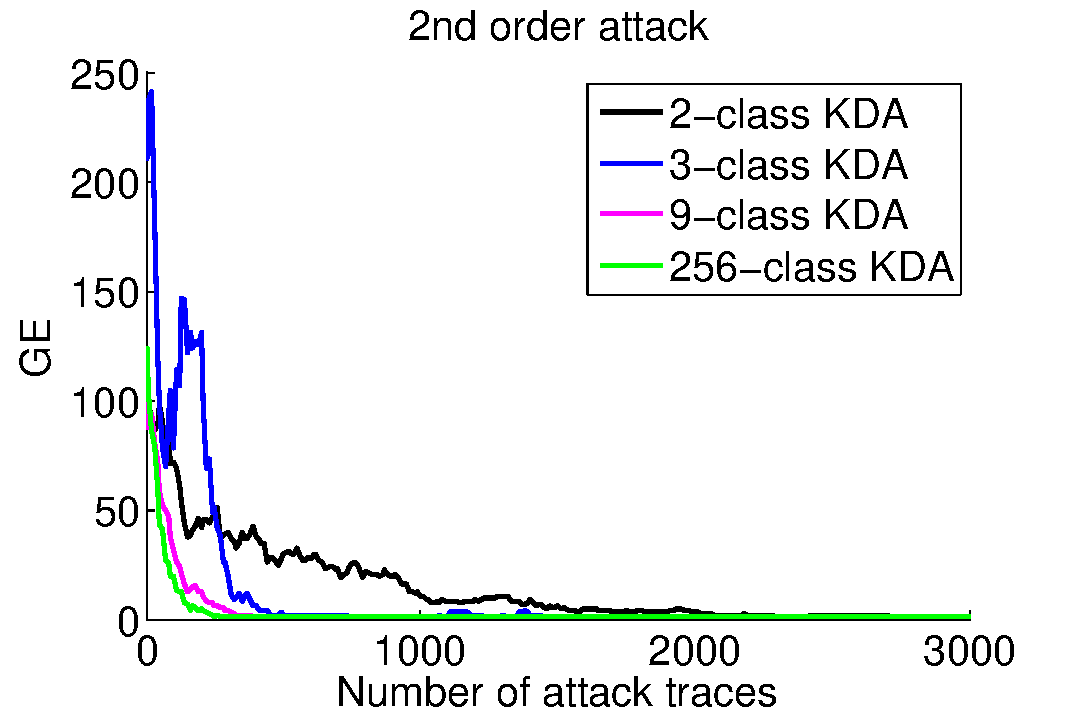
\includegraphics[width=.5\textwidth]{../Figures/CARDIS2016/2order_classes_TA.pdf}}
\subfigure[]{\label{fig:numClasses-3order}
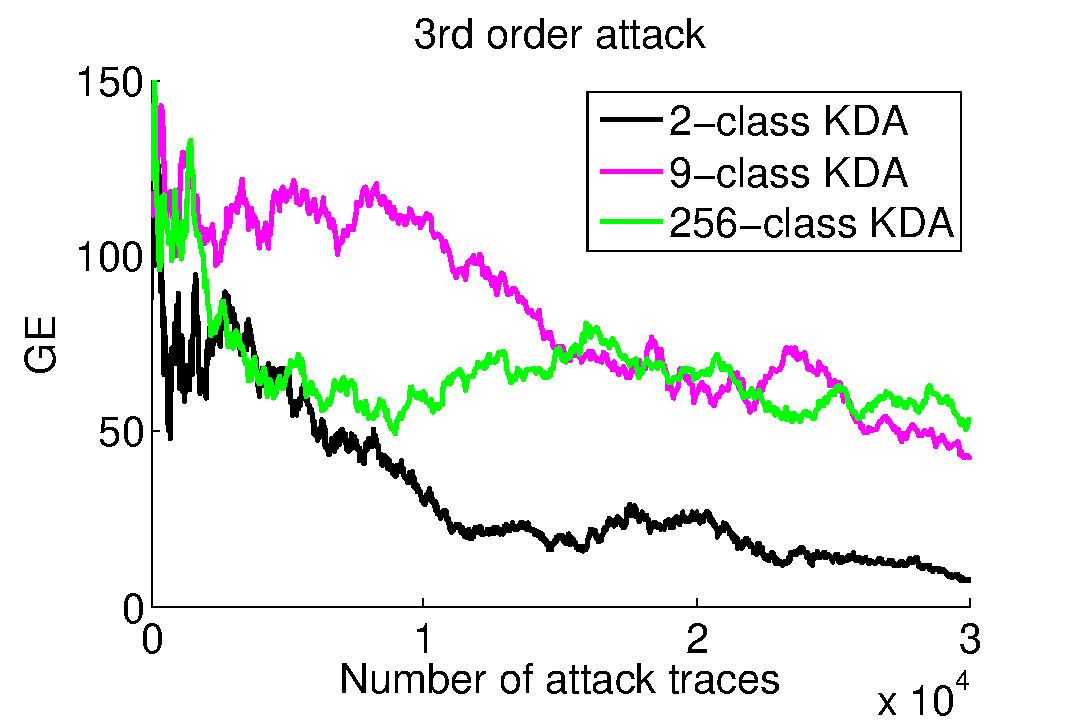
\includegraphics[width=.5\textwidth]{../Figures/CARDIS2016/3order_new.pdf}}
\caption[Comparison between 2-class,3-class, 9-class and 256-class KDA.]{Comparison between 2-class,3-class, 9-class and 256-class KDA in $2$nd-order context \subref{fig:numClasses-2order} and in $3$rd-order context \subref{fig:numClasses-3order}. For $2$nd-order the KDA is efficient in providing separability between 256 classes, allowing an optimal attack. In $3$rd-order context the training data are not enough to succeed the 256-class learning phase. Decreasing the number of classes to be distinguished raises the efficiency of the learning problem and thus of the attack.}\label{fig:numClasses}
\end{figure}

As discussed in Sec.~\ref{sec:LDA}, the LDA, and by consequence the KDA, looks for a subspace of the feature space to optimally separate some given classes. The performance of the KDA algorithm raises with the size $\nbTraces$ of the training set. Nevertheless, the number of examples might be bounded by the acquisition context, and even when the $\nbTraces$ can be very high, it may be interesting to minimize it since the KDA complexity is $O(\nbTraces^3)$. A trade-off must therefore be found between accuracy and efficiency. Assuming that the size of the training set  is fixed to $\nbTraces$, which controls the efficiency, a way to gain in accuracy may be found by appropriately adjusting the number of classes to distinguish: intuitively, the more examples per class, the more accurate the detection of a separating subspace. Then, if the total number of training traces is fixed, in order to raise the number of traces per class, a smaller number of classes must be considered. To do so, a non-injective model $m(\cdot)$ can be introduced, to create a smaller set of labels $m(\sensVarSet)$ from the initial set $\sensVarSet$. The reduced number of classes, \emph{i.e.} the number of labels assigned to the training set after applying the model $m$, will be denoted by $W$ (it is the cardinality of $m(\sensVarSet)$).  As discussed in Sections~\ref{sec:sensVar} and \ref{sec:leakage_model}, a widely-accepted power-consumption model for side-channel traces is provided by the Hamming Weight ($\HW$) function, thus we consider and experimentally compare the following models:
\begin{itemize}
\item 2-class model ($W = 2$)
\begin{equation*}
\begin{cases}
m(\sensVar) =0 \mbox{ if } \HW(\sensVar)<4 \\
m(\sensVar) =1 \mbox{ if } \HW(\sensVar)\geq 4
\end{cases}
\end{equation*}

\item 3-class model ($W = 3$)
\begin{equation*}
\begin{cases}
m(\sensVar) =0 \mbox{ if } \HW(\sensVar)<4 \\
m(\sensVar) =1 \mbox{ if } \HW(\sensVar) = 4\\
m(\sensVar) =2 \mbox{ if } \HW(\sensVar)>4 
\end{cases}
\end{equation*}

\item 9-class model ($W = 9$)
\begin{equation*}
m(\sensVar) = \HW(\sensVar) \mbox{ .} 
\end{equation*}

\end{itemize}

\begin{remark}\label{rem:numComp}
The separating subspace given by the KDA has maximal dimension $(W-1)$, \emph{i.e.} $Q\leq (W-1)$ in point 4 of Sec.~\ref{sec:KDA}. When $W=2$ a single discriminant component $\extract^{\mathrm{KDA}}_1$ is available. In this case we cannot run a bivariate template attack as we do with other extractors, thus we run a univariate one. \\
\end{remark}


A balanced training set of size $\nbTraces=9000$ (instead of 8960) has been used to run the experiments for $2$-class, $3$-class and $9$-class KDA. For the sake of consistency\footnote{A different approach is analysed in Sec.~\ref{sec:asymmetric}.} between the pre-processing phase and the attack phase, when a non-injective model is applied to the labels of the training set to reduce the number of classes, the same model is exploited to run the template attack: $W$ templates (one per each class) are estimated from the profiling set and compared to the attack traces. Thus, results of the experimental comparison of these different multi-class approaches depicted in  Fig.~\ref{fig:numClasses} are obtained using different template attacks. It may be remarked that as $W$ decreases the efficiency of the attack is supposed to decrease as well, because each attack trace contributes in distinguishing the right key $\keyRandVar^\star$ only from a growing-size set of indistinguishable hypotheses. 


 
In $2$nd-order context, it can be observed in Fig.~\ref{fig:numClasses} that the KDA is provided with sufficient training traces to succeed a 256-class separation, which allows the finest characterization of the leakage, and leads as expected (see Remark~\ref{rem:efficiency}), to the most efficient template attack. Moving to the $3$-rd order context, the available training set is insufficient to make the multi-class approach succeed; nevertheless, turning the problem into a 2-class problem turns out to be a good strategy to trade extraction accuracy for attack efficiency.






\begin{figure}
\centering
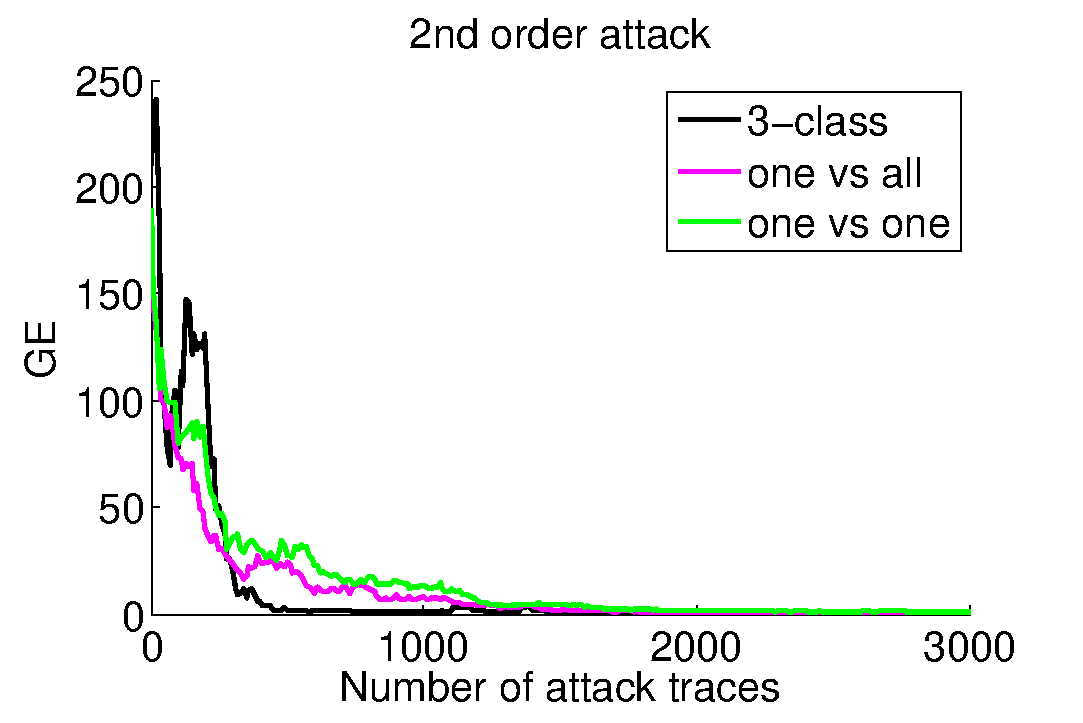
\includegraphics[width=.5\textwidth]{../Figures/CARDIS2016/2order_MULT.pdf}
\caption[KDA: comparison between multi-class, one vs one and one vs all approaches.]{Performance of template attacks run over 3-class KDA subspaces: multi-class, one vs one and one vs all approaches compared.}\label{fig:3multi-class}
\end{figure}

An idea to avoid an excessive reduction of the number of separable classes $W$ is given in the machine learning literature: it consists in treating the $W$-class problem as  multiple 2-class problems. Two different \emph{modus operandi} exist: the \emph{one-vs-one} and the \emph{one-vs-all}. When applied to our context, the one-vs-one approach determines for each pair of classes the 1-dimensional subspace that best separates them and exploits all the obtained subspaces to run an attack (for $W$ classes we obtain ${W}\choose{2}$ dimensions and we run a ${W}\choose{2}$-variate template attack). The one-vs-all approach looks for dimensions that best separate each class from all the others (obtaining $W$ projections in total).\\


We tested this approach in the 3-class case: in this way the one-vs-one and the one-vs-all approaches provide both 3 dimensions that we use to run a $3$-variate template attack, and that we compare to the $3$-class multi-class approach with bivariate template attack. Our experimental results, summed up in Fig.~\ref{fig:3multi-class}, show that no gain  is obtained by the 2-classes strategies.\footnote{We think that is result is quite data-dependant, so the use of such an approach is not discouraged in general.} We therefore chose to not consider them for the higher-order experiments.



\subsection{Asymmetric Preprocessing/Attack Approach}\label{sec:asymmetric}

\begin{figure}
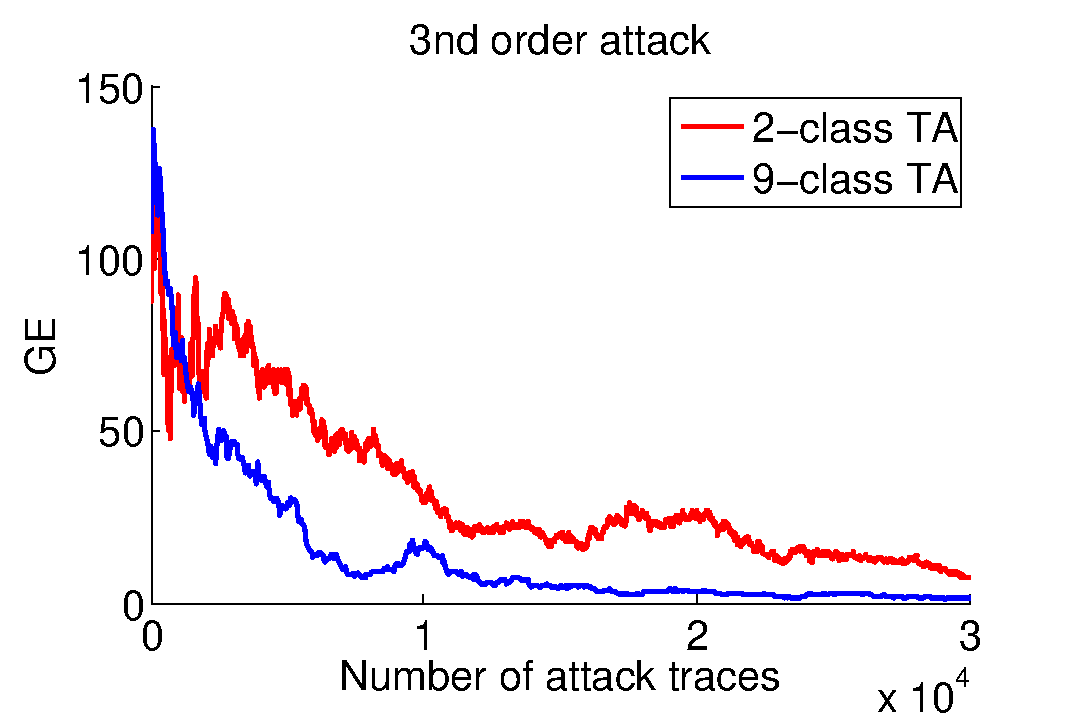
\includegraphics[width=.5\textwidth]{../Figures/CARDIS2016/3order_2_9.pdf} 
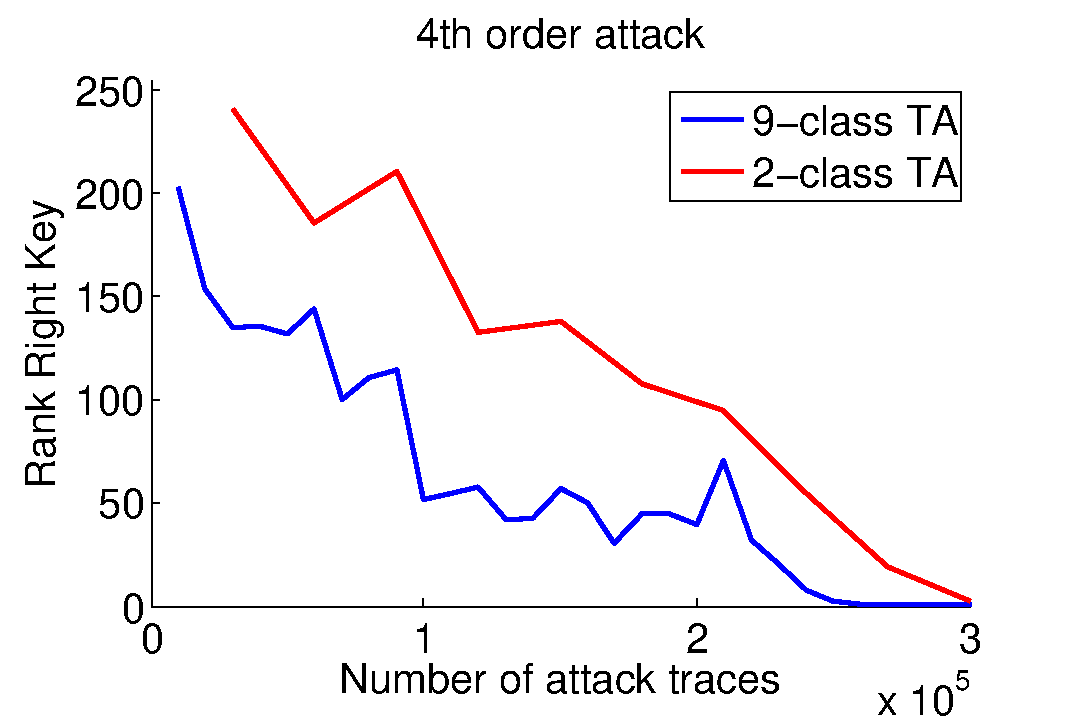
\includegraphics[width=.5\textwidth]{../Figures/CARDIS2016/4order_2_9.pdf} 
\caption[KDA preprocessing performance for  $3$rd-order and $4$th-order template attack]{Left: guessing entropy (over 10 independent tests) for a 2-class and a 9-class $3$rd-order template attack. Right: right key rank of a 2-class and a 9-class $4$th-order template attack.}\label{fig:3-4}
\end{figure}
In previous section we appealed a consistency principle to justify the choice of running a $W$-class template attack after a $W$-class KDA extraction. Here we propose a different reasoning: the consistency principle does not grant that an extractor $\extract^{\mathrm{KDA}}$ trained with $W$ classes is not able to separate $W^\prime$ classes with $W^\prime > W$. As seen in Sec.~~\ref{sec:implicit}, an extractor $\extract^{\mathrm{KDA}}$ always implicitly performs a weighed sum, via the implicit coefficients, of centred products of time samples. If $\extract^{\mathrm{KDA}}$ is effective, the implicit coefficients which have the highest magnitude must correspond to time samples corresponding to the manipulation of sensitive data (\emph{e.g.} the variable shares when masking is applied). This property is not necessarily related to the number of classes used to train the extractor.\\

Based on the reasoning above, we experienced the $3$rd-order and the $4$th-order attacks in an asymmetric way: as preprocessing we performed a $2$-class KDA, which gave best performances compared to others in the 3rd-order context (Fig.~\ref{fig:numClasses-3order}), then we performed  a $9$-class template attack, in order to raise the accuracy of the profiling and the efficiency of the attack.  The results are depicted in Fig.~\ref{fig:3-4} and confirm that, for our experimental data, this approach is sound: in both cases, using the same extractor trained with 2 classes and the same attack traces, the $9$-class approach outperforms the $2$-class one.
 
%\begin{remark}
%We choose to run the $9$-class instead of the $256$-class template attack in order to raise the accuracy of the profiling phase, being limited in terms of profiling traces. 
%\end{remark}


\subsection{Comparison with Projection Pursuits}\label{sec:comparisonPP}

To get a fair comparison, we run the PP algorithm (see Sec.~\ref{sec:PP_description}) over the same training set used to evaluate the KDA in Sec.\ref{sec:practice}. The best results in the $2$nd-order context were obtained with the HW model (\emph{i.e.}  $\lvert \sensVarSet \rvert=9$). In this case $T_{det}$ is fixed to $0.7$. Since 4 training sets are required, the 9000 training traces are split in 4 equally-sized groups.  Experimental observations allowed to fix  $W_{len}=5$, consequently suggesting $minWS=1$, $maxWS = 15$ and consistent global and local movements and resizes.
 Given the heuristic asset of the algorithm, we run it 1000 times for $d=2$ and for $d=3$. An overview of the global behaviour of the obtained results is depicted in Figs~\ref{fig:PP2} and \ref{fig:PP3}: the lower parts of the figures show the sum of the 1000 outputs of the algorithm.
  We recall that each coordinate of $\AAlpha$ is set to 1 for the windows identified to be of interest, and to 0 elsewhere, so for each time sample the sum of the values ($0$ or $1$) assigned by the $1000$ attempts give an intuition about its likelihood to be considered as interesting by the PP method. It can be observed that in the $2$-nd order case (Fig.~\ref{fig:PP2}) the results are excellent: 100\% of the tests highlight an informative part of the two clock-cycles where the sensitive shares are manipulated.\footnote{It can be observed that the regions selected by $\extract^{PP}$ correspond to those for which the $\extract^{KDA}$ exhibits the highest magnitude implicit coefficients (Fig.~\ref{fig:mu}, upper-triangular part on the right)}
It means that $\extract^{PP}(\vaLeakVec)$ always contains information about $\sensRandVar$ and a successful attack can be mounted over such extracted traces. The efficiency of such an attack depending on many factors, there is no interest in comparing it to the performances of the template attacks run in $2$nd-order context using $\extract^{KDA}$ and depicted in Fig.~\ref{fig:numClasses-2order}.
As it may be observed in Fig.~\ref{fig:PP3}, in the $3$-rd order case the experimental results are completely different: almost no $\AAlpha$ selects the clock-cycle where the second share is manipulated. Thus in this case the PP approach fails: $\extract^{PP}(\vaLeakVec)$ does not contain information about $\sensRandVar$, so any attack launched over the extracted traces would fail, while $\extract^{KDA}$ still allows successful attacks in $3$rd-order and $4$th-order case, as depicted in Fig.~\ref{fig:3-4}.\\

\begin{figure}[t]
\subfigure[]{\label{fig:PP2}
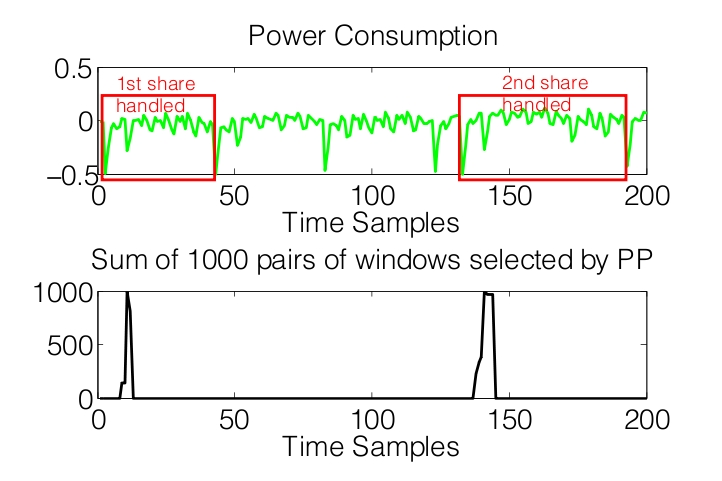
\includegraphics[width=.5\textwidth]{../Figures/CARDIS2016/secondOrderPP_gimp.jpg}}
\subfigure[]{\label{fig:PP3}
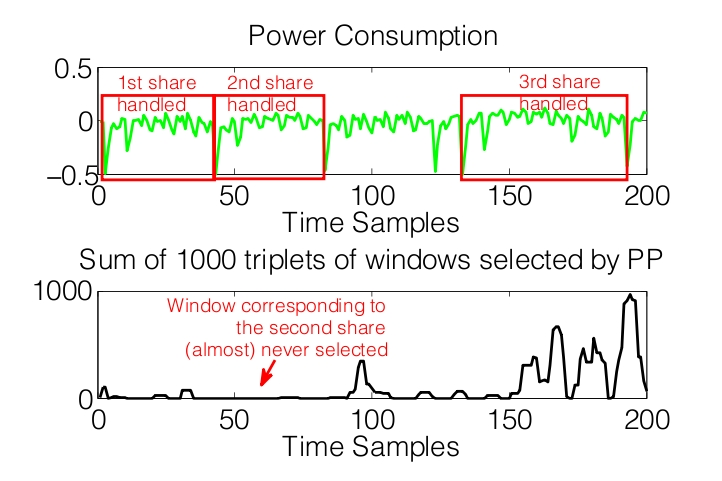
\includegraphics[width=.5\textwidth]{../Figures/CARDIS2016/thirdOrderPP_gimp.jpg}}
\caption[Overview of Projection Pursuit outputs in $2$nd-order and $3$rd-order context.]{\subref{fig:PP2} Overview of PP outputs in $2$nd-order context. \subref{fig:PP3} Overview of PP outputs in $3$rd-order context. }
\end{figure}

We conclude that the KDA approach is a valuable alternative to the PP one, especially in contexts where the training set size is bounded and independent from the order $d$ of the attack.


%----------------------------------------------------------------------------------------
%	SECTION 5
%----------------------------------------------------------------------------------------
\section{Conclusions and Drawbacks}\label{sec:KDAdrawbacks}
In this chapter we analysed the use of the KDA method to extract small-sized informative features from side-channel acquisitions protected by a $(d-1)$th-order masking countermeasure. The KDA naturally extends  the LDA technique to the generic $d$th-order context. It requires the choice of a so-called kernel function. We proposed to choose a polynomial kernel function, because it perfectly fit the necessary condition to perform a  higher-order side-channel attack. Indeed, in this way the obtained extractor  provides the linear combination of all possible $d$th-degree monomial in the time coordinates of the traces, which maximises the SNR.  The main obstacle to the problems of PoI selection and dimensionality reduction in higher-order side-channel context is given by the fact the size of the space containing all possible $d$th-degree monomials explodes combinatorially while $d$ grows. Nevertheless, the KDA only implicitly operates in such a space, by means of a so-called kernel trick, implying that its complexity is independent from the order $d$. This property represents the main advantage of the KDA. Experiments described in this chapter in $2$nd-order, $3$rd-order and $4$th-order contexts confirmed that such an approach is effective. Anyway, this approach presents some drawbacks, discussed hereafter. 

\paragraph*{Regularization hyper-parameter} First of all, to apply this methodology an attacker has to deal with choice of a regularization hyper-parameter. This problem still appears unsolved in subsequent studies \cite{zhou2017novel}. 
\paragraph*{Non scalability to big training set} The computational cost of the optimization problem is affected by the number of side-channel traces it uses for the training. This obliges the attacker to find a good trade-off between the efficiency of the information extraction, its accuracy and the efficiency of the underlying attack, through a careful choice of the target classification model. Besides the computational cost, the size of the training set also affects the memory complexity of the dimensionality reduction model: training traces cannot be forgot after the training of $\extract^{\mathrm{KDA}}$ but have to be stored in memory. Bishop assigned to this characteristic with the adjective \emph{memory-based} \cite[Chapter~6]{christopher2006pattern}. Indeed, observing the form of the KDA extractor \eqref{eq:projectionKDA}, one can remark that each time sample of each training trace makes part of the parameters defining it, together with the entries of the eigenvectors $\nununu_1, \dots, \nununu_\numEigenvectors$. This might be a surprisingly huge number of parameters: for example in our experiments, the extractor $\extract^{\mathrm{KDA}}:\mathbb{R}^200\rightarrow\mathbb{R}^2$ constructed exploiting a $8960$-sized training set counts $(8960+2)\times200 = 1.792.400$ parameters. In the case of 2nd-order context, this number is much higher than the number of implicit coefficients assigned to all possible $2$nd-degree monomials in time samples, which is ${{200+2-1}\choose{2}} = 20100$.

\paragraph*{Misalignment Affection} The KDA being an efficient way to perform LDA in a larger feature space, it maintains the same weakness than the LDA to trace misalignment, discussed in Sec.~\ref{sec:misalignment}.  
\paragraph*{Two-Phased Approach}
The approach presented in this chapter (and in Chapter~\ref{ChapterLinear} as well) is characterised by being two-phased. Indeed, a preliminary training has to be done in order to construct the extractor $\extract$, that plays the role of preprocessing for side-channel traces. Then, such an extractor is applied to traces and a second profiling phase has to be performed in order to construct the generative model that characterises the Gaussian template attack. In the specific case of KDA, these two preliminary phases demand the exploitation of two different profiling set, as discussed in Sec.~\ref{sec:experimental_setup}, which might be a great disadvantage in contexts where profiling acquisitions are bounded. Anyway, there is a general greater disadvantage of this two-phased approach, which is the fact that the preprocessing part, aiming in reducing the dimensionality of the samples, inevitably reduces the information held by side-channel traces, and such a pruning is mainly guided by some prior assumptions about the form informative parts of the data takes. For example, the fact that the polynomial kernel function proposed in this chapter fits with the necessary condition given in Property~\ref{property:poly}, does not guaranty that a linear combination of $d$th-degree monomials is the most efficient preprocessing to extract sensitive information from the traces. Even when such a linear combination is chosen to maximise a precise well-chosen criterion, in case of KDA it is chosen to maximise the SNR of projected data, through the Rayleigh quotient condition, this criterion does not directly coincide with the goal of the attack, \ie construct a classifier that allows to optimally distinguish the right secret key of the attacked algorithm from the wrong ones, or at least that allow to optimally classify the sensitive variable value handled during the acquisition of the attack traces. This same drawback of dimensionality reduction techniques is present in any preprocessing strategy, \eg in realignment techniques: a preprocessing aiming at realign data has a partial objective (the resynchronization) that does not coincide with the final goal of the attack, thus inject a risk of degrading data quality with respect to the final goal. This remark about data preprocessing is not specific to SCA context. Indeed, it is the one that pushed the Machine Learning community to develop the Deep Learning (DL) branch: as we will see in next chapter, and as anticipated in Sec.~\ref{sec:NN_intro}, DL models are conceived to integrate in a unique optimising process (the learning phase) any preprocessing with the model construction. 
